\section*{Problema 04}

\textbf{En este problema comparán varios esquemas de inicialización para al algoritmo de agrupamiento k-medias}

\begin{itemize}
    \item \textbf{El esquema de inicialización aleratorio o `random'.}
    \item \textbf{El esquema de inicialización `k-means++'.}
    \item \textbf{Proponga su propio esquema de inicialización.}
\end{itemize}

\textbf{Para $k \in \{2, 4, 8, 16, 32\}$ y para los 3 esquemas de inicialización, ejecute el algoritmo k-medias para la imagen a color \file{Colorful-Flowers.jpg} y obtenga la representación comprimida. Considere cada pixel como un punto en 3 dimensiones.}

\subsection*{Punto 01}

\textbf{Ejecute cada inicialización 5 veces con diferentes semillas y muestre en una gráfica el mínimo y la media de la función obejtivo de k-medias como una función de k.}

En la figura \ref{fig:problema_04_mean_and_minimum} se muestra el promedio y mínimo de la función objetivo de inicializador del método de k-means. En esta se visualiza que la tendencia de las dos es semejante. La diferencia promedio entre la media y mínimo es 1.0729. Comparado con el orden de magnitud de la función de costo este valor es muy pequeño. Por lo que tomar el mínimo un promedio de los resultados no varia mucho en las predicciones de cada modelo.

\begin{figure}[H]
    \centering
    \begin{subfigure}{16cm}
        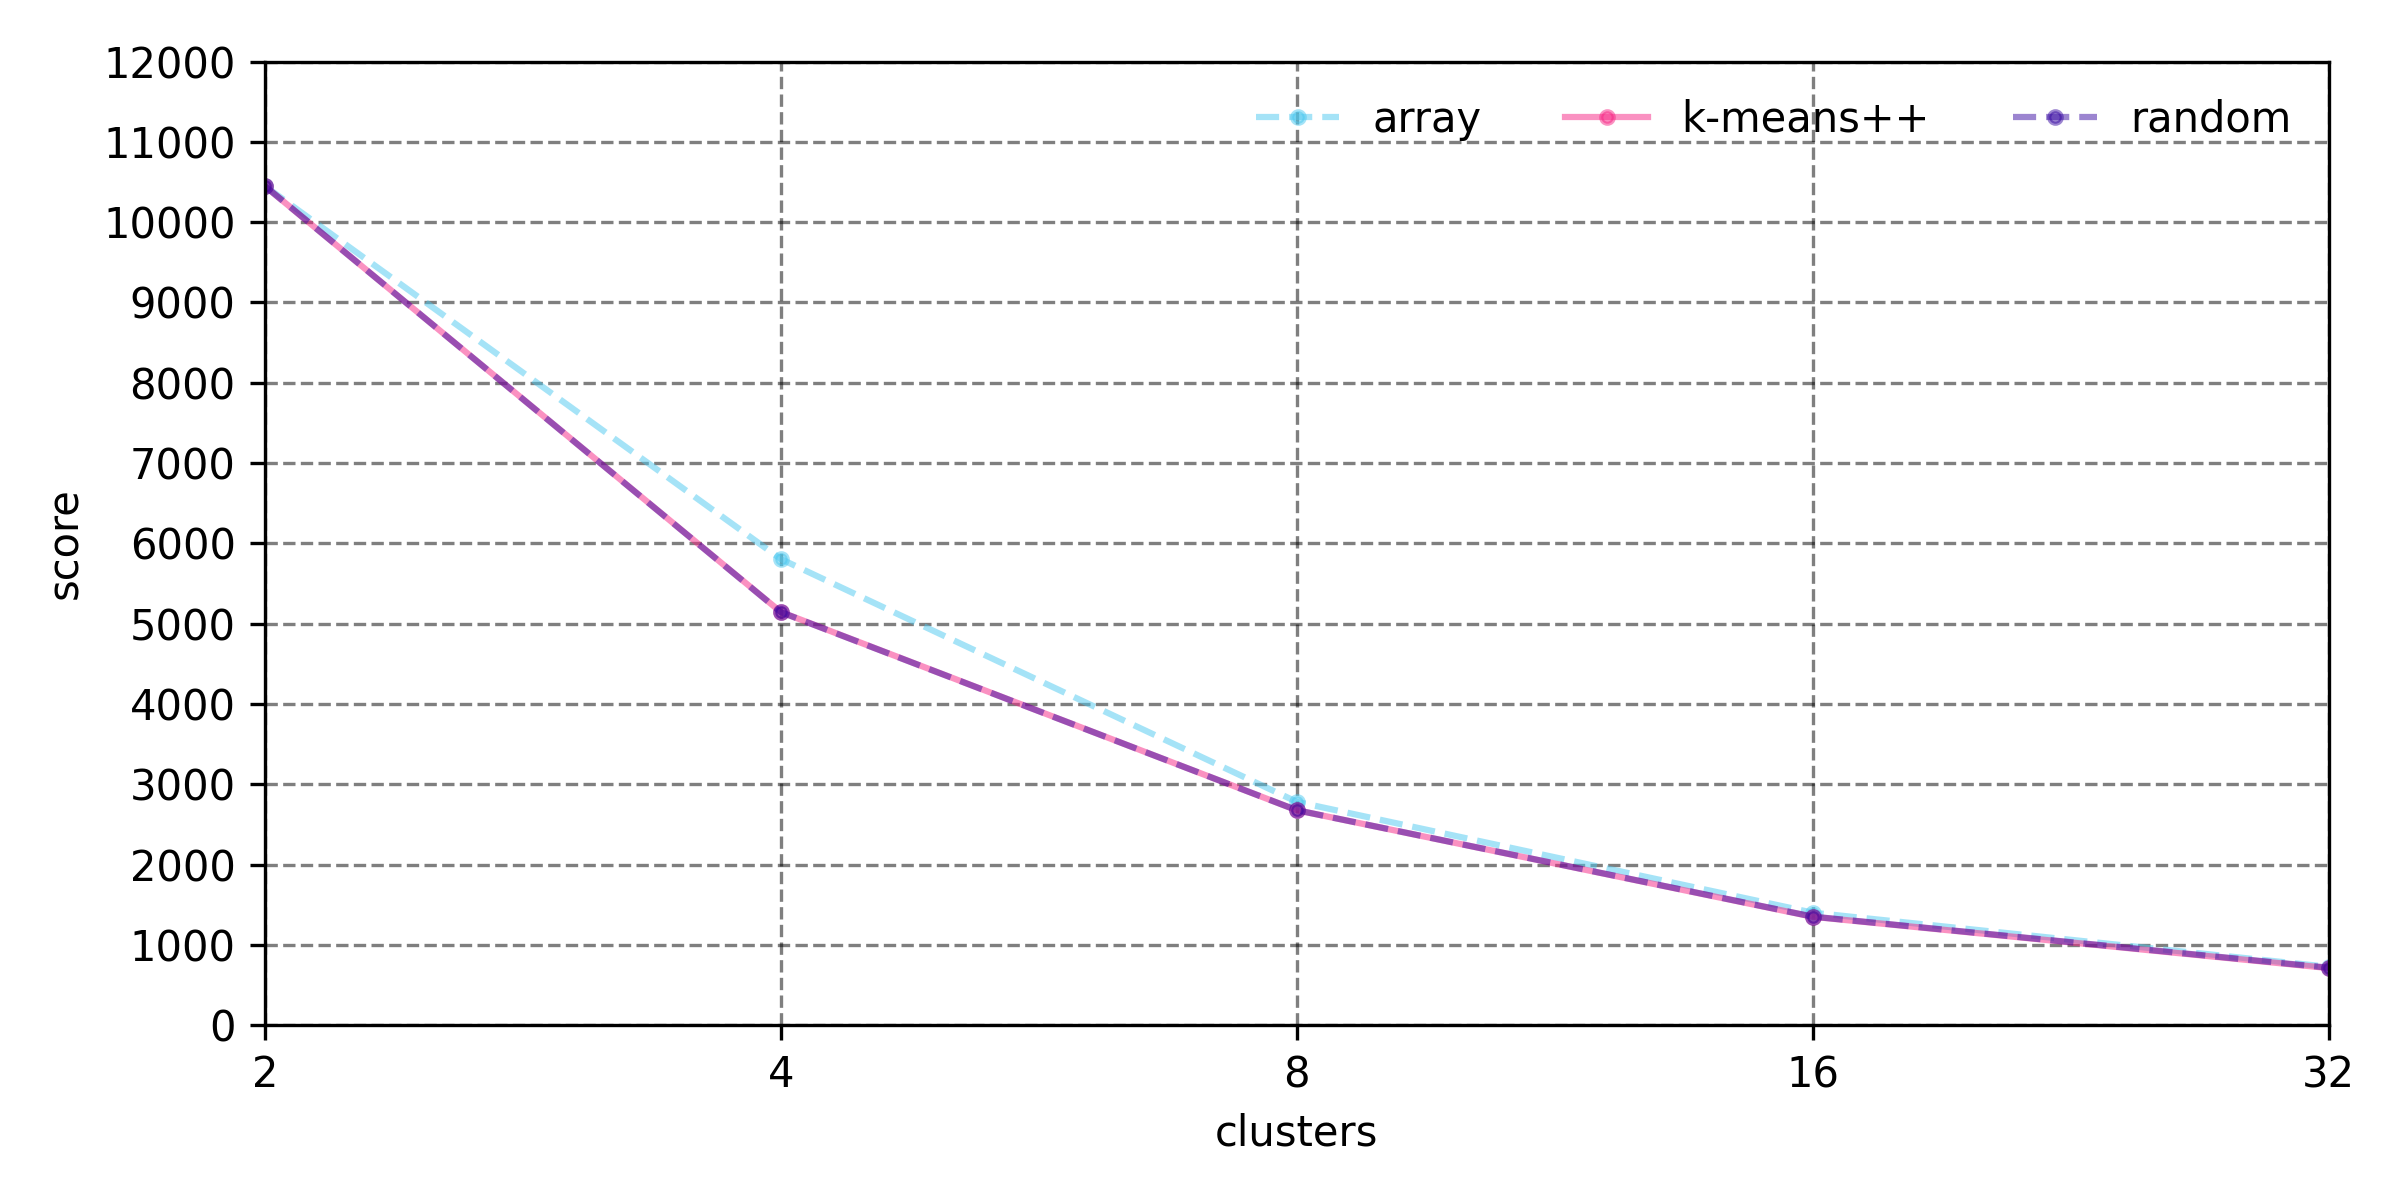
\includegraphics[width=16cm]{Graphics/Problema_04/mean_scores.png}
        \caption{Promedios de la función objetivo.}
    \end{subfigure}
    \begin{subfigure}{16cm}
        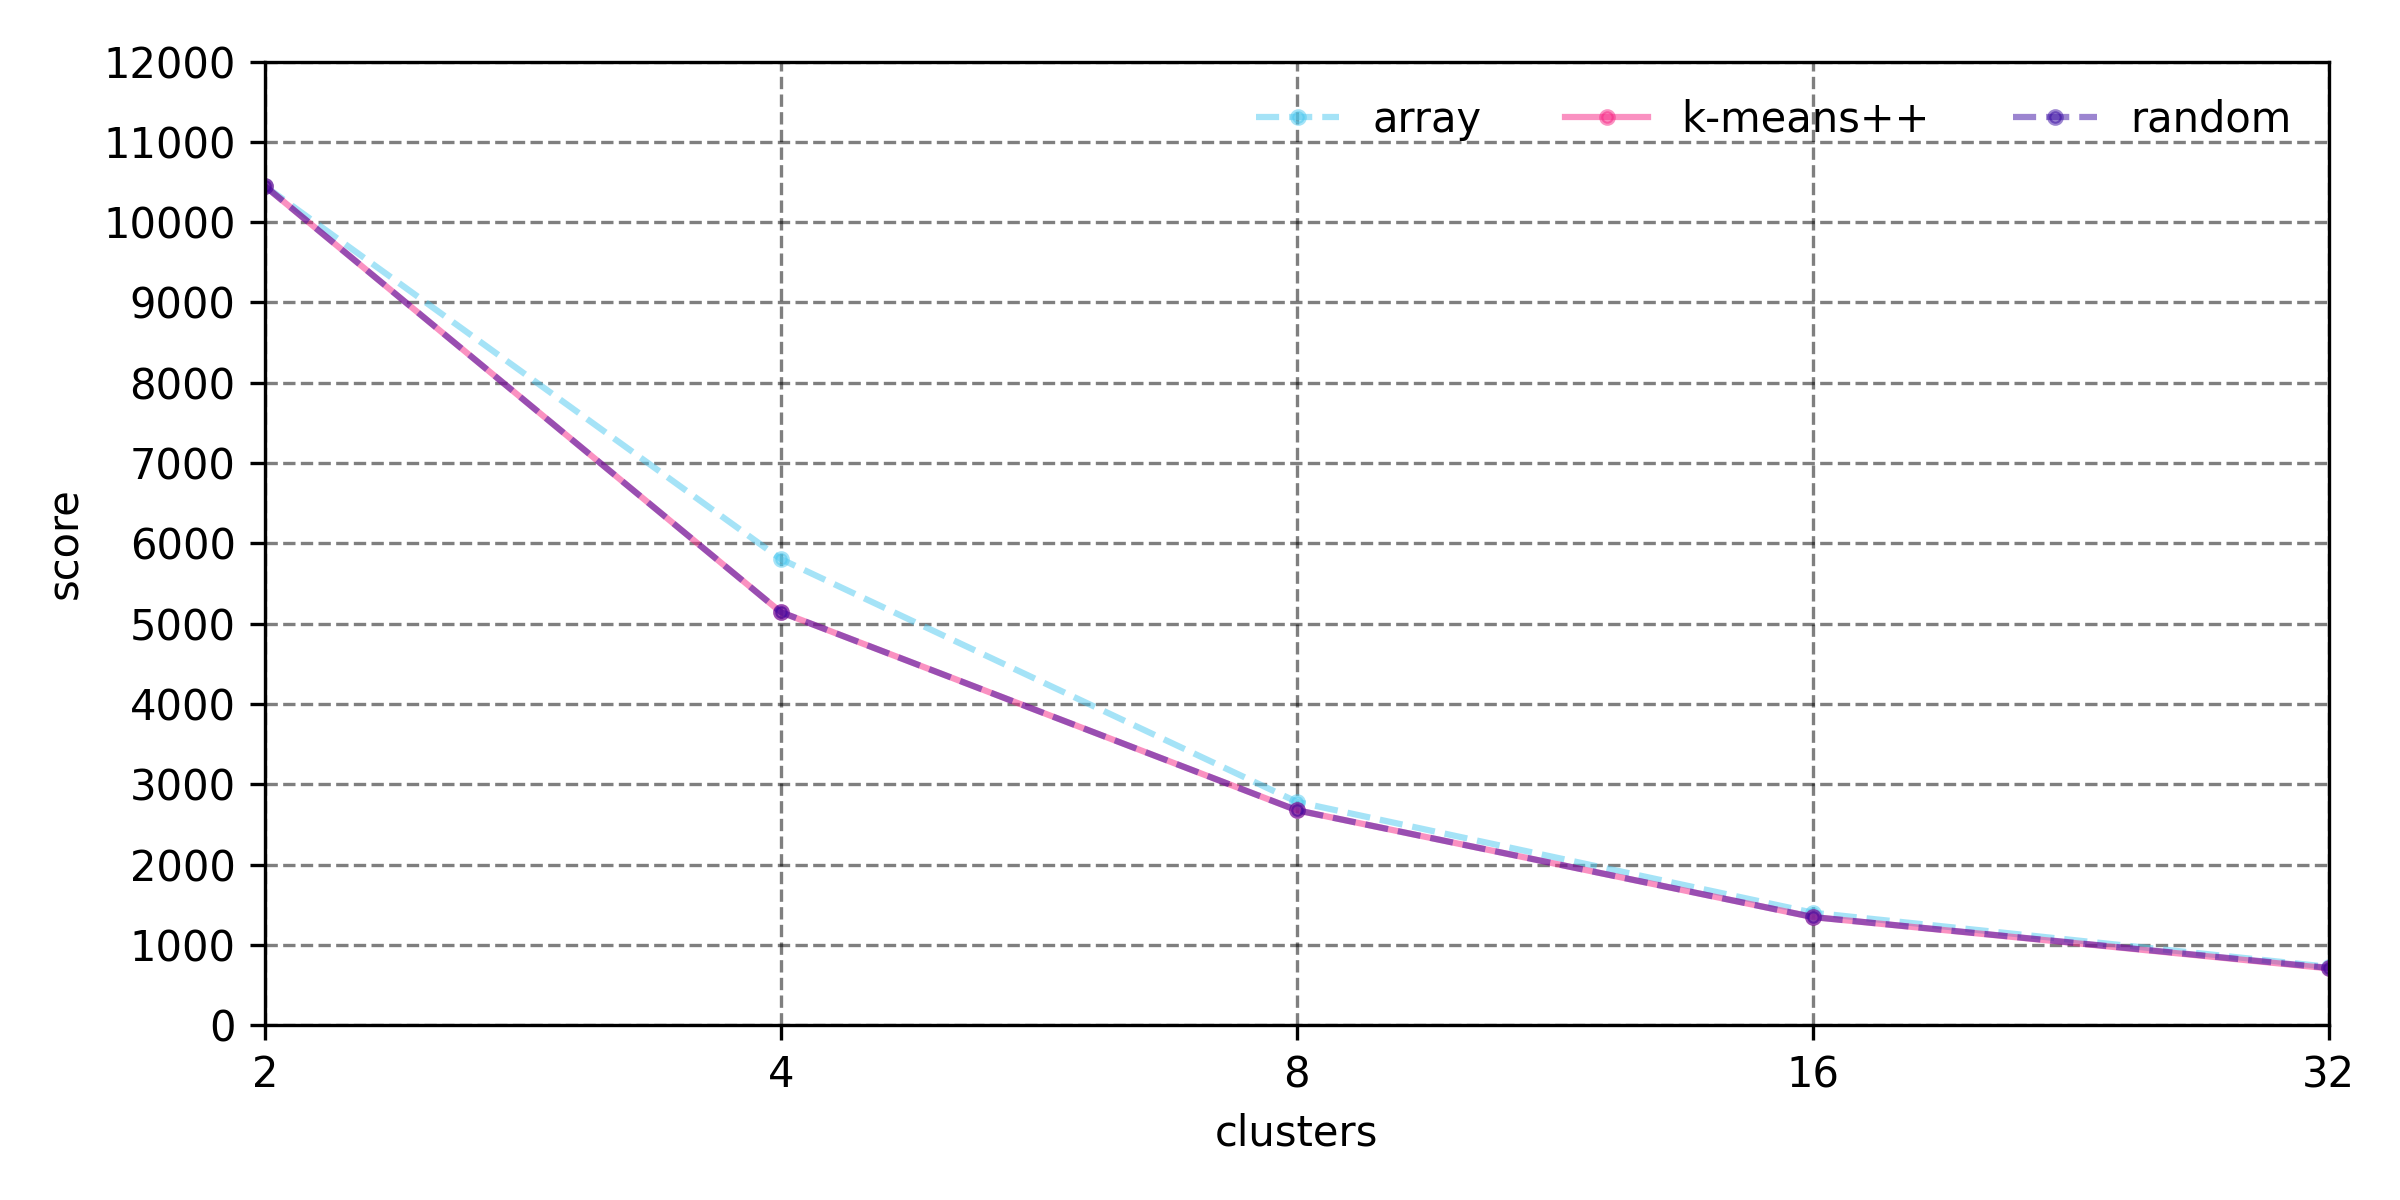
\includegraphics[width=16cm]{Graphics/Problema_04/minimum_scores.png}
        \caption{Mínimo de la función de objetivo.}
    \end{subfigure}
    \caption{Promedios y mínimo de la función objetivo de cada inicializador dado en el método de k-means.}
    \label{fig:problema_04_mean_and_minimum}
\end{figure}
\subsection*{Punto 02}

\textbf{Calcula y muestra el índice Fowlkes Mallows score (FM) usando el conjunto de entrenamiento. Muestra en una gráfica FM como una función de k, y comenta al respecto. Qué valor de k maximiza este criterio?}

En la figura \ref{fig:fowlkes_score} se visualiza el ínidice de Fowlkes Mallows para cada k calculada con el conjunto de entrenamiento. El índice de Fowlkes Mallows sigue una forma semejante a la figura \ref{fig:problema_05_minimum_score}. La diferencia se encuentra en el orden de magnitud de los valores de cada score obtenido. Si se quisiera máximizar el índice de Fowlkes Mallows se usaría k=2. Ya que para este valor se obtiene el valor máximo del índice.

\begin{figure}[H]
    \centering
    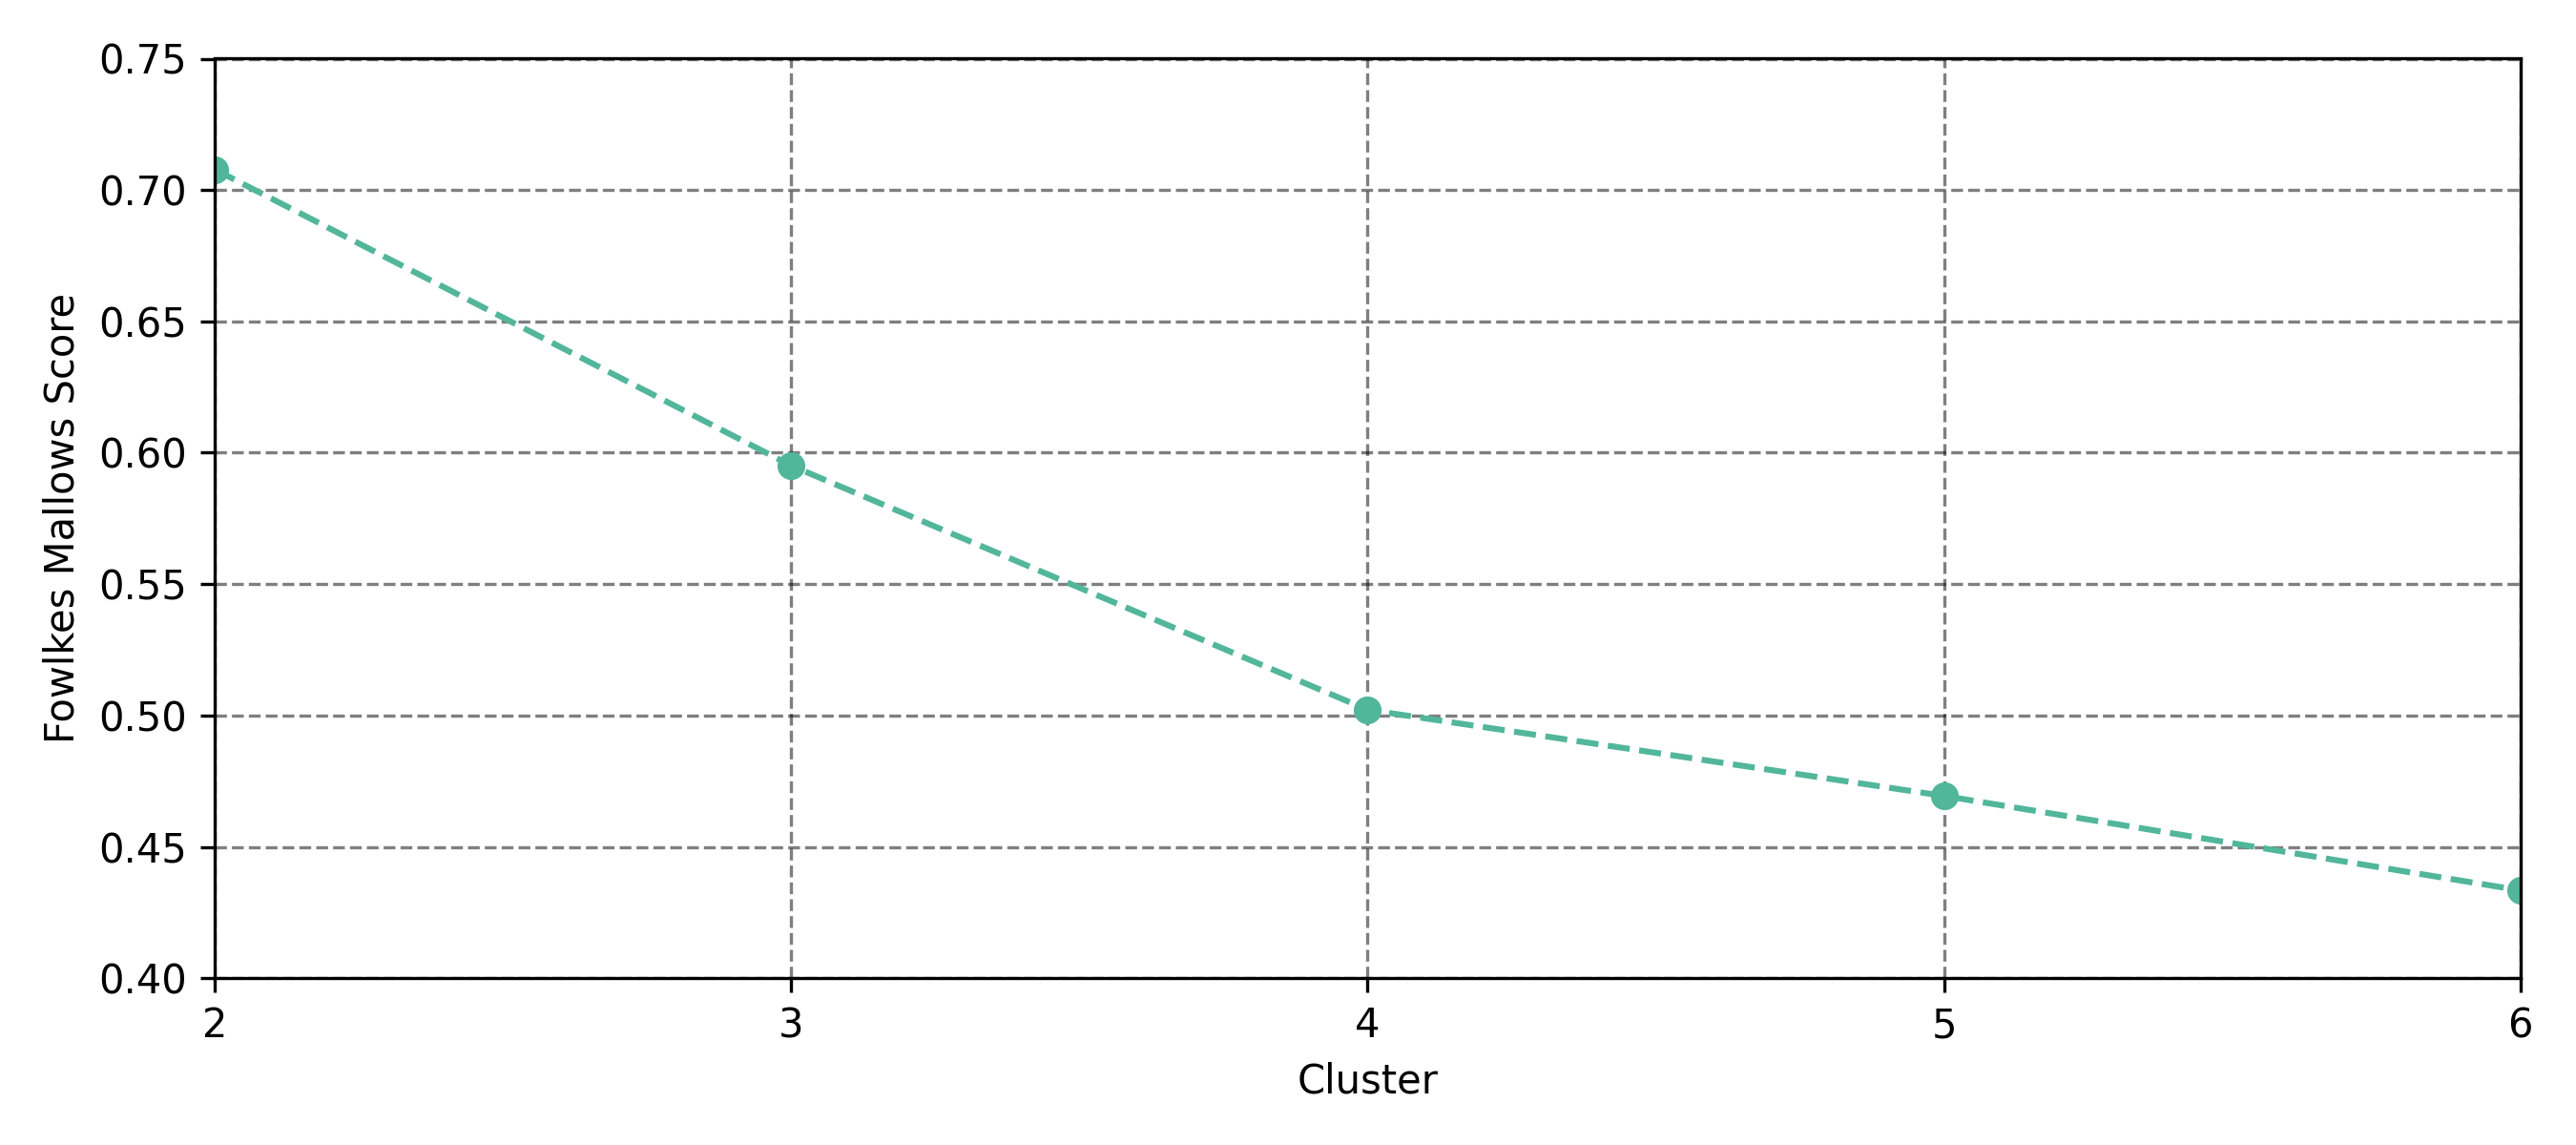
\includegraphics[width=15cm]{Graphics/Problema_05/fowlkes_mallows_score.png}
    \caption{Índice de Fowlkes Mallows obtenido a partir de los resultados usando el conjunto de entrenamiento del dataset \file{creditcard.csv}.}
    \label{fig:fowlkes_score}
\end{figure}